\batchmode
\documentclass[csgeo,tcc]{unipampa}
\RequirePackage{ifthen}

                                          
\usepackage[utf8]{inputenc} 
\usepackage[T1]{fontenc}                                    
\usepackage{graphicx}                                       
\usepackage{chngcntr}                                       
\counterwithout{figure}{chapter}                            % contagem contínua das figuras [Não especificado nas normas, porém de preferência do autor]
\usepackage{times}                                          
\usepackage{mathptmx}                                       
\usepackage[alf,abnt-emphasize=bf]{abntex2cite}	            
\usepackage{ragged2e}                                       
\usepackage{booktabs}                                       
\usepackage[table]{xcolor}                                  
\usepackage[labelsep=endash]{caption}                       
\usepackage{amsmath}
\usepackage{xcolor}
\usepackage{verbatim}
\usepackage{pdflscape}
\usepackage{lscape}

%
\providecommand{\rot}[1]{\nabla \times \vec{\textrm{#1}}}%
\providecommand{\MT}{magnetotelúrico }                                               % mt -> magnetotelúrico%
\providecommand{\citar}[1]{\textcolor{red}{#1}}                                      % marca em vermelho locais para correção%
\providecommand{\en}[1]{\textit{#1}}                                                 % marca em italico termos em ingles%
\providecommand{\ven}[1]{\vec{\textrm{#1}}}                                          % Coloca o vetor em cima da incognita%
\providecommand{\parct}[1]{\dfrac{\partial \vec{\textrm{#1}}}{\partial t}}           % derivada Parcial de t%
\providecommand{\parctto}[1]{\dfrac{\partial^2 \vec{\textrm{#1}}}{\partial t^2}}     % derivada Parcial de t

%
\providecommand{\codnum}[1]{\begin{flushright} \normalsize (#1) \end{flushright}}    %numera os scripts%
\providecommand{\codbox}[1]{{\fontfamily{pcr}\selectfont #1}}                        %ambiente para escrever codigo fonte. OBS deve estar dentro do ambiente quote%
\providecommand{\cc}[1]{\textcolor{gray}{\textit{\# #1}}}                            %cor para comentarios (cinza)%
\providecommand{\f}[1]{\textbf{\textcolor{OliveGreen}{#1}}}                          %cor para funcoes (verde)%
\providecommand{\cl}[1]{\textbf{\textcolor{BurntOrange}{#1}}}                        %cor para classes (laranja)%
\providecommand{\ob}[1]{\textcolor{Blue}{#1}}%
\providecommand{\st}[1]{\textcolor{OliveGreen}{#1}}%
\providecommand{\ini}{>{}>{}> \, }                                                   % produz >>>%
\providecommand{\init}{>{}>{}> \, \, \, \, \,}                                       % produz >>> tabulado 1vez%
\providecommand{\initt}{>{}>{}> \, \, \, \, \, \, \, \, \,}                          % produz >>> tabulado 2vez%
\providecommand{\inittt}{>{}>{}> \, \, \, \, \, \, \, \, \, \, \, \, \,}             % produz >>> tabulado 3vez


\title{Desenvolvimento de Software livre para processamentos de Dados Magnetotelúricos}                              


\author{Garcia}{Patrick Rogger}                                    


\advisor[Prof.~Dr.]{Oliveira}{Vinicius Abreu de}                        
	\coadvisor[Prof\textsuperscript{a}.~Dr.\textsuperscript{a}.]{Matos}{Andréa Cristina Lima dos Santos}   
	%
\renewcommand{\coadvisorname}{Co-orientadora}


\cutter{} 
\banca[Prof.~Dr.]{Frigo}{Éverton}			                
	\inst{Universidade Federal do Pampa}					    


\banca[Prof.~Dr.]{Gonçalves}{Ítalo}                           
	\inst{Universidade Federal do Pampa}	                    


\defesa{DIA}{MÊS}{ANO}                                    


\location{Caçapava do Sul}{RS}                              


\keyword{Magnetotelúrico}
	\keyword{Python3}
	\keyword{Software Livre}


\sloppy                                                       




\usepackage[latin1]{inputenc}



\makeatletter

\makeatletter
\count@=\the\catcode`\_ \catcode`\_=8 
\newenvironment{tex2html_wrap}{}{}%
\catcode`\<=12\catcode`\_=\count@
\newcommand{\providedcommand}[1]{\expandafter\providecommand\csname #1\endcsname}%
\newcommand{\renewedcommand}[1]{\expandafter\providecommand\csname #1\endcsname{}%
  \expandafter\renewcommand\csname #1\endcsname}%
\newcommand{\newedenvironment}[1]{\newenvironment{#1}{}{}\renewenvironment{#1}}%
\let\newedcommand\renewedcommand
\let\renewedenvironment\newedenvironment
\makeatother
\let\mathon=$
\let\mathoff=$
\ifx\AtBeginDocument\undefined \newcommand{\AtBeginDocument}[1]{}\fi
\newbox\sizebox
\setlength{\hoffset}{0pt}\setlength{\voffset}{0pt}
\addtolength{\textheight}{\footskip}\setlength{\footskip}{0pt}
\addtolength{\textheight}{\topmargin}\setlength{\topmargin}{0pt}
\addtolength{\textheight}{\headheight}\setlength{\headheight}{0pt}
\addtolength{\textheight}{\headsep}\setlength{\headsep}{0pt}
\setlength{\textwidth}{349pt}
\newwrite\lthtmlwrite
\makeatletter
\let\realnormalsize=\normalsize
\global\topskip=2sp
\def\preveqno{}\let\real@float=\@float \let\realend@float=\end@float
\def\@float{\let\@savefreelist\@freelist\real@float}
\def\liih@math{\ifmmode$\else\bad@math\fi}
\def\end@float{\realend@float\global\let\@freelist\@savefreelist}
\let\real@dbflt=\@dbflt \let\end@dblfloat=\end@float
\let\@largefloatcheck=\relax
\let\if@boxedmulticols=\iftrue
\def\@dbflt{\let\@savefreelist\@freelist\real@dbflt}
\def\adjustnormalsize{\def\normalsize{\mathsurround=0pt \realnormalsize
 \parindent=0pt\abovedisplayskip=0pt\belowdisplayskip=0pt}%
 \def\phantompar{\csname par\endcsname}\normalsize}%
\def\lthtmltypeout#1{{\let\protect\string \immediate\write\lthtmlwrite{#1}}}%
\newcommand\lthtmlhboxmathA{\adjustnormalsize\setbox\sizebox=\hbox\bgroup\kern.05em }%
\newcommand\lthtmlhboxmathB{\adjustnormalsize\setbox\sizebox=\hbox to\hsize\bgroup\hfill }%
\newcommand\lthtmlvboxmathA{\adjustnormalsize\setbox\sizebox=\vbox\bgroup %
 \let\ifinner=\iffalse \let\)\liih@math }%
\newcommand\lthtmlboxmathZ{\@next\next\@currlist{}{\def\next{\voidb@x}}%
 \expandafter\box\next\egroup}%
\newcommand\lthtmlmathtype[1]{\gdef\lthtmlmathenv{#1}}%
\newcommand\lthtmllogmath{\dimen0\ht\sizebox \advance\dimen0\dp\sizebox
  \ifdim\dimen0>.95\vsize
   \lthtmltypeout{%
*** image for \lthtmlmathenv\space is too tall at \the\dimen0, reducing to .95 vsize ***}%
   \ht\sizebox.95\vsize \dp\sizebox\z@ \fi
  \lthtmltypeout{l2hSize %
:\lthtmlmathenv:\the\ht\sizebox::\the\dp\sizebox::\the\wd\sizebox.\preveqno}}%
\newcommand\lthtmlfigureA[1]{\let\@savefreelist\@freelist
       \lthtmlmathtype{#1}\lthtmlvboxmathA}%
\newcommand\lthtmlpictureA{\bgroup\catcode`\_=8 \lthtmlpictureB}%
\newcommand\lthtmlpictureB[1]{\lthtmlmathtype{#1}\egroup
       \let\@savefreelist\@freelist \lthtmlhboxmathB}%
\newcommand\lthtmlpictureZ[1]{\hfill\lthtmlfigureZ}%
\newcommand\lthtmlfigureZ{\lthtmlboxmathZ\lthtmllogmath\copy\sizebox
       \global\let\@freelist\@savefreelist}%
\newcommand\lthtmldisplayA{\bgroup\catcode`\_=8 \lthtmldisplayAi}%
\newcommand\lthtmldisplayAi[1]{\lthtmlmathtype{#1}\egroup\lthtmlvboxmathA}%
\newcommand\lthtmldisplayB[1]{\edef\preveqno{(\theequation)}%
  \lthtmldisplayA{#1}\let\@eqnnum\relax}%
\newcommand\lthtmldisplayZ{\lthtmlboxmathZ\lthtmllogmath\lthtmlsetmath}%
\newcommand\lthtmlinlinemathA{\bgroup\catcode`\_=8 \lthtmlinlinemathB}
\newcommand\lthtmlinlinemathB[1]{\lthtmlmathtype{#1}\egroup\lthtmlhboxmathA
  \vrule height1.5ex width0pt }%
\newcommand\lthtmlinlineA{\bgroup\catcode`\_=8 \lthtmlinlineB}%
\newcommand\lthtmlinlineB[1]{\lthtmlmathtype{#1}\egroup\lthtmlhboxmathA}%
\newcommand\lthtmlinlineZ{\egroup\expandafter\ifdim\dp\sizebox>0pt %
  \expandafter\centerinlinemath\fi\lthtmllogmath\lthtmlsetinline}
\newcommand\lthtmlinlinemathZ{\egroup\expandafter\ifdim\dp\sizebox>0pt %
  \expandafter\centerinlinemath\fi\lthtmllogmath\lthtmlsetmath}
\newcommand\lthtmlindisplaymathZ{\egroup %
  \centerinlinemath\lthtmllogmath\lthtmlsetmath}
\def\lthtmlsetinline{\hbox{\vrule width.1em \vtop{\vbox{%
  \kern.1em\copy\sizebox}\ifdim\dp\sizebox>0pt\kern.1em\else\kern.3pt\fi
  \ifdim\hsize>\wd\sizebox \hrule depth1pt\fi}}}
\def\lthtmlsetmath{\hbox{\vrule width.1em\kern-.05em\vtop{\vbox{%
  \kern.1em\kern0.8 pt\hbox{\hglue.17em\copy\sizebox\hglue0.8 pt}}\kern.3pt%
  \ifdim\dp\sizebox>0pt\kern.1em\fi \kern0.8 pt%
  \ifdim\hsize>\wd\sizebox \hrule depth1pt\fi}}}
\def\centerinlinemath{%
  \dimen1=\ifdim\ht\sizebox<\dp\sizebox \dp\sizebox\else\ht\sizebox\fi
  \advance\dimen1by.5pt \vrule width0pt height\dimen1 depth\dimen1 
 \dp\sizebox=\dimen1\ht\sizebox=\dimen1\relax}

\def\lthtmlcheckvsize{\ifdim\ht\sizebox<\vsize 
  \ifdim\wd\sizebox<\hsize\expandafter\hfill\fi \expandafter\vfill
  \else\expandafter\vss\fi}%
\providecommand{\selectlanguage}[1]{}%
\makeatletter \tracingstats = 1 
\providecommand{\Iota}{\textrm{J}}
\providecommand{\Alpha}{\textrm{A}}
\providecommand{\Chi}{\textrm{X}}
\providecommand{\Kappa}{\textrm{K}}
\providecommand{\Mu}{\textrm{M}}
\providecommand{\Rho}{\textrm{R}}
\providecommand{\Zeta}{\textrm{Z}}
\providecommand{\Epsilon}{\textrm{E}}
\providecommand{\omicron}{\textrm{o}}
\providecommand{\Eta}{\textrm{H}}
\providecommand{\Tau}{\textrm{T}}
\providecommand{\Omicron}{\textrm{O}}
\providecommand{\Nu}{\textrm{N}}
\providecommand{\Beta}{\textrm{B}}


\begin{document}
\pagestyle{empty}\thispagestyle{empty}\lthtmltypeout{}%
\lthtmltypeout{latex2htmlLength hsize=\the\hsize}\lthtmltypeout{}%
\lthtmltypeout{latex2htmlLength vsize=\the\vsize}\lthtmltypeout{}%
\lthtmltypeout{latex2htmlLength hoffset=\the\hoffset}\lthtmltypeout{}%
\lthtmltypeout{latex2htmlLength voffset=\the\voffset}\lthtmltypeout{}%
\lthtmltypeout{latex2htmlLength topmargin=\the\topmargin}\lthtmltypeout{}%
\lthtmltypeout{latex2htmlLength topskip=\the\topskip}\lthtmltypeout{}%
\lthtmltypeout{latex2htmlLength headheight=\the\headheight}\lthtmltypeout{}%
\lthtmltypeout{latex2htmlLength headsep=\the\headsep}\lthtmltypeout{}%
\lthtmltypeout{latex2htmlLength parskip=\the\parskip}\lthtmltypeout{}%
\lthtmltypeout{latex2htmlLength oddsidemargin=\the\oddsidemargin}\lthtmltypeout{}%
\makeatletter
\if@twoside\lthtmltypeout{latex2htmlLength evensidemargin=\the\evensidemargin}%
\else\lthtmltypeout{latex2htmlLength evensidemargin=\the\oddsidemargin}\fi%
\lthtmltypeout{}%
\makeatother
\setcounter{page}{1}
\onecolumn

% !!! IMAGES START HERE !!!

{\newpage\clearpage
\lthtmlinlinemathA{tex2html_wrap_inline4044}%
$ \rho $%
\lthtmlinlinemathZ
\lthtmlcheckvsize\clearpage}

{\newpage\clearpage
\lthtmlinlinemathA{tex2html_wrap_inline4048}%
$ y$%
\lthtmlinlinemathZ
\lthtmlcheckvsize\clearpage}

{\newpage\clearpage
\lthtmlfigureA{listofabbrv257}%
\begin{listofabbrv}{UNIPAMPA}
\par
\item[API]          {\textit{Application Programming Interface}}
        \item[ASCII]        {\textit{American Standard Code for Information Interchange}}
        \item[CPU]          {\textit{Central Processing Unit}}
        \item[CWI]          {\textit{Centrum Wishunde \& Informatica}}
        \item[GEOMA]        {Grupo de Geomagnetismo}
        \item[INPE]         {Instituto Nacional de Pesquisas Espaciais}
        \item[MT]           {Magnetotelúrico}
        \item[1D]           {Uma Dimensão}
        \item[2D]           {Duas Dimensões}
        \item[3D]           {Três Dimensões}
        \item[TE]           {Transversal Elétrico}
        \item[TM]           {Transversal Magnético}
        \item[TS]           {\textit{Time Series}}
\end{listofabbrv}%
\lthtmlfigureZ
\lthtmlcheckvsize\clearpage}

{\newpage\clearpage
\lthtmlfigureA{listofsymbols273}%
\begin{listofsymbols}{$\alpha\beta\pi\omega$}
       \item[$\sigma$]                  Condutividade Elétrica
       \item[$\rho$]                    Resistividade Elétrica
       \item[$V$]                       Diferença de Potencial
       \item[$i$]                       Corrente Elétrica
       \item[$R$]                       Resistência Elétrica
       \item[$A$]                       Área
       \item[$L$]                       Comprimento
       \item[$\nabla \times$]           Rotacional
       \item[$\nabla \cdot$]            Divergente
       \item[$\vec{\textrm{E}}$]                 Campo Elétrico
       \item[$\vec{\textrm{H}}$]                 Campo Magnetizante
       \item[$\vec{\textrm{B}}$]                 Campo Magnético
       \item[$\vec{\textrm{J}}$]                 Densidade de Corrente
       \item[$\vec{\textrm{D}}$]                 Campo de Deslocamento Elétrico
       \item[$\rho_f$]                  Densidade de Carga
       \item[$t$]                       Tempo
       \item[$\mu$]                     Permeabilidade Magnética
       \item[$\varepsilon$]             Permissividade Elétrica
\par
\end{listofsymbols}%
\lthtmlfigureZ
\lthtmlcheckvsize\clearpage}

\stepcounter{chapter}
\stepcounter{chapter}
\stepcounter{section}
\stepcounter{section}
\stepcounter{chapter}
\stepcounter{chapter}
\stepcounter{section}
{\newpage\clearpage
\lthtmlinlinemathA{tex2html_wrap_inline4285}%
$ mHz$%
\lthtmlinlinemathZ
\lthtmlcheckvsize\clearpage}

{\newpage\clearpage
\lthtmlinlinemathA{tex2html_wrap_inline4287}%
$ kHz$%
\lthtmlinlinemathZ
\lthtmlcheckvsize\clearpage}

{\newpage\clearpage
\lthtmlinlinemathA{tex2html_wrap_inline4289}%
$ Hz$%
\lthtmlinlinemathZ
\lthtmlcheckvsize\clearpage}

\stepcounter{section}
{\newpage\clearpage
\lthtmlinlinemathA{tex2html_wrap_inline4294}%
$ \sigma$%
\lthtmlinlinemathZ
\lthtmlcheckvsize\clearpage}

{\newpage\clearpage
\lthtmlinlinemathA{tex2html_wrap_indisplay4299}%
$\displaystyle V = R i$%
\lthtmlindisplaymathZ
\lthtmlcheckvsize\clearpage}

{\newpage\clearpage
\lthtmlinlinemathA{tex2html_wrap_inline4301}%
$ V$%
\lthtmlinlinemathZ
\lthtmlcheckvsize\clearpage}

{\newpage\clearpage
\lthtmlinlinemathA{tex2html_wrap_inline4303}%
$ i$%
\lthtmlinlinemathZ
\lthtmlcheckvsize\clearpage}

{\newpage\clearpage
\lthtmlinlinemathA{tex2html_wrap_inline4305}%
$ R$%
\lthtmlinlinemathZ
\lthtmlcheckvsize\clearpage}

{\newpage\clearpage
\lthtmlinlinemathA{tex2html_wrap_inline4307}%
$ \Omega$%
\lthtmlinlinemathZ
\lthtmlcheckvsize\clearpage}

{\newpage\clearpage
\lthtmlinlinemathA{tex2html_wrap_inline4309}%
$ m^2$%
\lthtmlinlinemathZ
\lthtmlcheckvsize\clearpage}

{\newpage\clearpage
\lthtmlinlinemathA{tex2html_wrap_inline4313}%
$ m$%
\lthtmlinlinemathZ
\lthtmlcheckvsize\clearpage}

{\newpage\clearpage
\lthtmlinlinemathA{tex2html_wrap_inline4317}%
$ \Omega m$%
\lthtmlinlinemathZ
\lthtmlcheckvsize\clearpage}

{\newpage\clearpage
\lthtmlinlinemathA{tex2html_wrap_indisplay4319}%
$\displaystyle \rho = \dfrac{R A}{L}\, \, \, ;\, \, \, \, \, \, \, \, \, \, \, \, \, \,  R = \dfrac{V}{i}$%
\lthtmlindisplaymathZ
\lthtmlcheckvsize\clearpage}

{\newpage\clearpage
\lthtmlinlinemathA{tex2html_wrap_inline4329}%
$ 100 \, \Omega m$%
\lthtmlinlinemathZ
\lthtmlcheckvsize\clearpage}

{\newpage\clearpage
\lthtmlinlinemathA{tex2html_wrap_inline4331}%
$ 3000 \, \Omega m $%
\lthtmlinlinemathZ
\lthtmlcheckvsize\clearpage}

\stepcounter{section}
{\newpage\clearpage
\lthtmlinlinemathA{tex2html_wrap_indisplay4339}%
$\displaystyle \nabla \times \vec{\textrm{E}}=-\frac{\partial \vec{\textrm{B}}}{\partial t}$%
\lthtmlindisplaymathZ
\lthtmlcheckvsize\clearpage}

{\newpage\clearpage
\lthtmlinlinemathA{tex2html_wrap_indisplay4341}%
$\displaystyle \nabla \times \vec{\textrm{H}} = \vec{\textrm{J}} + \frac{\partial \vec{\textrm{D}}}{\partial t}$%
\lthtmlindisplaymathZ
\lthtmlcheckvsize\clearpage}

{\newpage\clearpage
\lthtmlinlinemathA{tex2html_wrap_indisplay4343}%
$\displaystyle \nabla \cdot \vec{\textrm{B}} = 0$%
\lthtmlindisplaymathZ
\lthtmlcheckvsize\clearpage}

{\newpage\clearpage
\lthtmlinlinemathA{tex2html_wrap_indisplay4345}%
$\displaystyle \nabla \cdot \vec{\textrm{D}} = \rho_f$%
\lthtmlindisplaymathZ
\lthtmlcheckvsize\clearpage}

{\newpage\clearpage
\lthtmlfigureA{table495}%
\begin{table}             \begin{tabular*}{1cm}{p{0.05cm}p{0.1cm}p{10cm}}
               {\footnotesize$\vec{\textrm{E}}$}  & {\footnotesize$\rightarrow$} & {\footnotesize Campo Elétrico [$V/m$] }\\
               {\footnotesize$\vec{\textrm{B}}$}  & {\footnotesize$\rightarrow$} & {\footnotesize Campo Magnético [$T$] }\\
               {\footnotesize$\vec{\textrm{H}}$}  & {\footnotesize$\rightarrow$} & {\footnotesize Campo Magnetizante [$A/m$]} \\
               {\footnotesize$\vec{\textrm{J}}$}  & {\footnotesize$\rightarrow$} & {\footnotesize Densidade de Corrente [$A/m^2$]} \\
               {\footnotesize$\vec{\textrm{D}}$}  & {\footnotesize$\rightarrow$} & {\footnotesize Campo de Deslocamento Elétrico [$C/m^2$]} \\
               {\footnotesize$\rho_f$}            & {\footnotesize$\rightarrow$} & {\footnotesize Densidade de Carga [$C/m^3$]} \\
               {\footnotesize$t$\  }                & {\footnotesize$\rightarrow$} & {\footnotesize Tempo [$s$]}
             \end{tabular*}
\par
\end{table}%
\lthtmlfigureZ
\lthtmlcheckvsize\clearpage}

{\newpage\clearpage
\lthtmlinlinemathA{tex2html_wrap_indisplay4347}%
$\displaystyle \vec{\textrm{B}} = \mu \vec{\textrm{H}}$%
\lthtmlindisplaymathZ
\lthtmlcheckvsize\clearpage}

{\newpage\clearpage
\lthtmlinlinemathA{tex2html_wrap_indisplay4349}%
$\displaystyle \vec{\textrm{D}} = \varepsilon  \vec{\textrm{E}}$%
\lthtmlindisplaymathZ
\lthtmlcheckvsize\clearpage}

{\newpage\clearpage
\lthtmlinlinemathA{tex2html_wrap_indisplay4351}%
$\displaystyle \vec{\textrm{J}} = \sigma \vec{\textrm{E}}$%
\lthtmlindisplaymathZ
\lthtmlcheckvsize\clearpage}

{\newpage\clearpage
\lthtmlfigureA{table539}%
\begin{table}             \begin{tabular*}{1cm}{p{0.05cm}p{0.1cm}p{10cm}}
               {\footnotesize$\mu$}          & {\footnotesize$\rightarrow$} & {\footnotesize Permeabilidade Magnética [$H/m$] }\\
               {\footnotesize$\varepsilon$}  & {\footnotesize$\rightarrow$} & {\footnotesize Permissividade Elétrica [$F/m$] }\\
               {\footnotesize$\sigma$}       & {\footnotesize$\rightarrow$} & {\footnotesize Condutividade Elétrica [$S/m$]} \\
             \end{tabular*}
\par
\end{table}%
\lthtmlfigureZ
\lthtmlcheckvsize\clearpage}

{\newpage\clearpage
\lthtmlinlinemathA{tex2html_wrap_inline4353}%
$ \mu = 1,2566\textrm{x}10^{-6} H/m$%
\lthtmlinlinemathZ
\lthtmlcheckvsize\clearpage}

{\newpage\clearpage
\lthtmlinlinemathA{tex2html_wrap_inline4355}%
$ \varepsilon = 8,85
            \textrm{x}10^{-12} F/m$%
\lthtmlinlinemathZ
\lthtmlcheckvsize\clearpage}

{\newpage\clearpage
\lthtmlinlinemathA{tex2html_wrap_indisplay4357}%
$\displaystyle \nabla \times \vec{\textrm{E}} = - \mu \dfrac{\partial \vec{\textrm{H}}}{\partial t}$%
\lthtmlindisplaymathZ
\lthtmlcheckvsize\clearpage}

{\newpage\clearpage
\lthtmlinlinemathA{tex2html_wrap_indisplay4359}%
$\displaystyle \nabla \times \vec{\textrm{H}} = \sigma \vec{\textrm{E}} + \varepsilon \dfrac{\partial \vec{\textrm{E}}}{\partial t}$%
\lthtmlindisplaymathZ
\lthtmlcheckvsize\clearpage}

{\newpage\clearpage
\lthtmlinlinemathA{tex2html_wrap_inline4361}%
$ \mu$%
\lthtmlinlinemathZ
\lthtmlcheckvsize\clearpage}

{\newpage\clearpage
\lthtmlinlinemathA{tex2html_wrap_indisplay4362}%
$\displaystyle \dfrac{\partial (\nabla \times \vec{\textrm{H}})}{\partial t}$%
\lthtmlindisplaymathZ
\lthtmlcheckvsize\clearpage}

{\newpage\clearpage
\lthtmlinlinemathA{tex2html_wrap_indisplay4363}%
$\displaystyle = \dfrac{\partial (\sigma \vec{\textrm{E}})}{\partial t} + \dfrac{\partial}{\partial t} \bigg(\varepsilon \dfrac{\partial \vec{\textrm{E}}}{\partial t}\bigg)$%
\lthtmlindisplaymathZ
\lthtmlcheckvsize\clearpage}

{\newpage\clearpage
\lthtmlinlinemathA{tex2html_wrap_indisplay4364}%
$\displaystyle \dfrac{\nabla \times \partial \vec{\textrm{H}}}{\partial t}$%
\lthtmlindisplaymathZ
\lthtmlcheckvsize\clearpage}

{\newpage\clearpage
\lthtmlinlinemathA{tex2html_wrap_indisplay4365}%
$\displaystyle = \sigma \dfrac{\partial \vec{\textrm{E}}}{\partial t} + \varepsilon \dfrac{\partial^2 \vec{\textrm{E}}}{\partial t^2}$%
\lthtmlindisplaymathZ
\lthtmlcheckvsize\clearpage}

{\newpage\clearpage
\lthtmlinlinemathA{tex2html_wrap_indisplay4366}%
$\displaystyle \mu \dfrac{\nabla \times \partial \vec{\textrm{H}}}{\partial t}$%
\lthtmlindisplaymathZ
\lthtmlcheckvsize\clearpage}

{\newpage\clearpage
\lthtmlinlinemathA{tex2html_wrap_indisplay4367}%
$\displaystyle = \mu \sigma \dfrac{\partial \vec{\textrm{E}}}{\partial t} + \mu \varepsilon \dfrac{\partial^2 \vec{\textrm{E}}}{\partial t^2}$%
\lthtmlindisplaymathZ
\lthtmlcheckvsize\clearpage}

{\newpage\clearpage
\lthtmlinlinemathA{tex2html_wrap_indisplay4368}%
$\displaystyle -\dfrac{\mu}{\mu} \nabla \times \nabla \times \vec{\textrm{E}}$%
\lthtmlindisplaymathZ
\lthtmlcheckvsize\clearpage}

{\newpage\clearpage
\lthtmlinlinemathA{tex2html_wrap_indisplay4371}%
$\displaystyle - \nabla \times \nabla \times \vec{\textrm{E}} = \mu \sigma \dfrac{\partial \vec{\textrm{E}}}{\partial t} + \mu \varepsilon \dfrac{\partial^2 \vec{\textrm{E}}}{\partial t^2}$%
\lthtmlindisplaymathZ
\lthtmlcheckvsize\clearpage}

{\newpage\clearpage
\lthtmlinlinemathA{tex2html_wrap_indisplay4373}%
$\displaystyle \nabla \times \nabla \times \vec{\textrm{A}} = -\nabla^2 \vec{\textrm{A}} + \nabla(\nabla \cdot \vec{\textrm{A}})$%
\lthtmlindisplaymathZ
\lthtmlcheckvsize\clearpage}

{\newpage\clearpage
\lthtmlinlinemathA{tex2html_wrap_inline4375}%
$ \rho_f$%
\lthtmlinlinemathZ
\lthtmlcheckvsize\clearpage}

{\newpage\clearpage
\lthtmlinlinemathA{tex2html_wrap_indisplay4377}%
$\displaystyle \nabla \cdot \vec{\textrm{E}} = 0$%
\lthtmlindisplaymathZ
\lthtmlcheckvsize\clearpage}

{\newpage\clearpage
\lthtmlinlinemathA{tex2html_wrap_indisplay4379}%
$\displaystyle \nabla \times \nabla \times \vec{\textrm{E}} = -\nabla^2 \vec{\textrm{E}} + \nabla(\nabla \cdot \vec{\textrm{E}});\,\,\,\,\,\,\, \textrm{onde}\,\,\,\,\,\,\,   \nabla(\nabla \cdot \vec{\textrm{E}})=0$%
\lthtmlindisplaymathZ
\lthtmlcheckvsize\clearpage}

{\newpage\clearpage
\lthtmlinlinemathA{tex2html_wrap_indisplay4381}%
$\displaystyle \nabla^2 \vec{\textrm{E}} - \mu \sigma \dfrac{\partial \vec{\textrm{E}}}{\partial t} - \mu \varepsilon \dfrac{\partial^2 \vec{\textrm{E}}}{\partial t^2} = 0$%
\lthtmlindisplaymathZ
\lthtmlcheckvsize\clearpage}

{\newpage\clearpage
\lthtmlinlinemathA{tex2html_wrap_indisplay4383}%
$\displaystyle \nabla^2 \vec{\textrm{H}} - \mu \sigma \dfrac{\partial \vec{\textrm{H}}}{\partial t} - \mu \varepsilon \dfrac{\partial^2 \vec{\textrm{H}}}{\partial t^2} = 0$%
\lthtmlindisplaymathZ
\lthtmlcheckvsize\clearpage}

{\newpage\clearpage
\lthtmlinlinemathA{tex2html_wrap_indisplay4385}%
$\displaystyle \textrm{E}_x = A e^{-\imath k z} + \textrm{B} e^{\imath k z}$%
\lthtmlindisplaymathZ
\lthtmlcheckvsize\clearpage}

{\newpage\clearpage
\lthtmlinlinemathA{tex2html_wrap_indisplay4387}%
$\displaystyle \textrm{H}_y = \dfrac{k}{\omega \mu_0} (A e^{-\imath k z} + \textrm{B} e^{\imath k z})$%
\lthtmlindisplaymathZ
\lthtmlcheckvsize\clearpage}

{\newpage\clearpage
\lthtmlinlinemathA{tex2html_wrap_inline4389}%
$ k^2 = \imath \omega \mu_0 \sigma$%
\lthtmlinlinemathZ
\lthtmlcheckvsize\clearpage}

{\newpage\clearpage
\lthtmlinlinemathA{tex2html_wrap_inline4391}%
$ A$%
\lthtmlinlinemathZ
\lthtmlcheckvsize\clearpage}

{\newpage\clearpage
\lthtmlinlinemathA{tex2html_wrap_inline4393}%
$ B$%
\lthtmlinlinemathZ
\lthtmlcheckvsize\clearpage}

\stepcounter{section}
\stepcounter{subsection}
{\newpage\clearpage
\lthtmlinlinemathA{tex2html_wrap_indisplay4397}%
$\displaystyle \left (\begin{array}{c}
\textrm{E}_x\\
\textrm{E}_y
\end{array}\right)
=
\left (\begin{array}{cc}
\textrm{Z}_{xx} & \textrm{Z}_{xy}\\
\textrm{Z}_{yx} & \textrm{Z}_{yy}
\end{array}\right) \left (\begin{array}{c}
\textrm{H}_x\\
\textrm{H}_y
\end{array}\right)$%
\lthtmlindisplaymathZ
\lthtmlcheckvsize\clearpage}

{\newpage\clearpage
\lthtmlinlinemathA{tex2html_wrap_indisplay4399}%
$\displaystyle \textrm{E}_x (\omega)=\textrm{Z}_{xx}(\omega) \textrm{H}_{x}(\omega) + \textrm{Z}_{xy}(\omega) \textrm{H}_{y}(\omega)$%
\lthtmlindisplaymathZ
\lthtmlcheckvsize\clearpage}

{\newpage\clearpage
\lthtmlinlinemathA{tex2html_wrap_indisplay4401}%
$\displaystyle \textrm{E}_y (\omega)=\textrm{Z}_{yx}(\omega) \textrm{H}_{x}(\omega) + \textrm{Z}_{yy}(\omega) \textrm{H}_{y}(\omega)$%
\lthtmlindisplaymathZ
\lthtmlcheckvsize\clearpage}

\stepcounter{section}
\stepcounter{subsection}
{\newpage\clearpage
\lthtmlinlinemathA{tex2html_wrap_indisplay4405}%
$\displaystyle \textrm{Z}_{1 D} = \left ( \begin{array}{cc}
0 & \textrm{Z}_{xy} \\
-\textrm{Z}_{yx} & 0
\end{array}  \right)$%
\lthtmlindisplaymathZ
\lthtmlcheckvsize\clearpage}

{\newpage\clearpage
\lthtmlinlinemathA{tex2html_wrap_indisplay4407}%
$\displaystyle \textrm{Z}_{xy}(\omega) = \dfrac{\textrm{E}_x(\omega)}{\textrm{H}_y(\omega)} = \dfrac{\omega \mu_0}{k}$%
\lthtmlindisplaymathZ
\lthtmlcheckvsize\clearpage}

{\newpage\clearpage
\lthtmlinlinemathA{tex2html_wrap_indisplay4409}%
$\displaystyle \left | \dfrac{\textrm{E}_x(\omega)}{\textrm{H}_y(\omega)} \right | ^2 = \left | \dfrac{\omega \mu_0}{k} \right | ^2 = \dfrac{\omega \mu_0}{\sigma}$%
\lthtmlindisplaymathZ
\lthtmlcheckvsize\clearpage}

{\newpage\clearpage
\lthtmlinlinemathA{tex2html_wrap_indisplay4411}%
$\displaystyle \dfrac{1}{\sigma} = \dfrac{1}{\omega \mu_0} \left | \dfrac{\textrm{E}_x(\omega)}{\textrm{H}_y(\omega)} \right | ^2 = \rho$%
\lthtmlindisplaymathZ
\lthtmlcheckvsize\clearpage}

{\newpage\clearpage
\lthtmlinlinemathA{tex2html_wrap_indisplay4413}%
$\displaystyle \rho_a = \dfrac{1}{\omega \mu_0} \left | \textrm{Z} \right | ^2$%
\lthtmlindisplaymathZ
\lthtmlcheckvsize\clearpage}

{\newpage\clearpage
\lthtmlinlinemathA{tex2html_wrap_indisplay4415}%
$\displaystyle \phi = \textrm{arctg} \left ( \dfrac{\textrm{Im \, Z}}{\textrm{Re \, Z}} \right )$%
\lthtmlindisplaymathZ
\lthtmlcheckvsize\clearpage}

{\newpage\clearpage
\lthtmlinlinemathA{tex2html_wrap_inline4417}%
$ \delta_f[m])$%
\lthtmlinlinemathZ
\lthtmlcheckvsize\clearpage}

{\newpage\clearpage
\lthtmlinlinemathA{tex2html_wrap_inline4419}%
$ f[Hz]$%
\lthtmlinlinemathZ
\lthtmlcheckvsize\clearpage}

{\newpage\clearpage
\lthtmlinlinemathA{tex2html_wrap_inline4421}%
$ \rho_a[\Omega.m]$%
\lthtmlinlinemathZ
\lthtmlcheckvsize\clearpage}

{\newpage\clearpage
\lthtmlinlinemathA{tex2html_wrap_indisplay4422}%
$\displaystyle \delta_\omega$%
\lthtmlindisplaymathZ
\lthtmlcheckvsize\clearpage}

{\newpage\clearpage
\lthtmlinlinemathA{tex2html_wrap_indisplay4423}%
$\displaystyle = \dfrac{1}{\textrm{Re}(k)}$%
\lthtmlindisplaymathZ
\lthtmlcheckvsize\clearpage}

{\newpage\clearpage
\lthtmlinlinemathA{tex2html_wrap_indisplay4425}%
$\displaystyle = \dfrac{1}{\textrm{Re} \left (\sqrt{\imath \omega \mu_0 \sigma} \right)}$%
\lthtmlindisplaymathZ
\lthtmlcheckvsize\clearpage}

{\newpage\clearpage
\lthtmlinlinemathA{tex2html_wrap_indisplay4427}%
$\displaystyle = \sqrt{ \left (\dfrac{2}{\omega \mu_0 \sigma} \right )}$%
\lthtmlindisplaymathZ
\lthtmlcheckvsize\clearpage}

{\newpage\clearpage
\lthtmlinlinemathA{tex2html_wrap_indisplay4429}%
$\displaystyle \delta_\omega = \sqrt{\frac{2}{\omega \mu \sigma}} \longrightarrow \delta_f \approx 500  \sqrt{\frac{\rho_a}{f}}$%
\lthtmlindisplaymathZ
\lthtmlcheckvsize\clearpage}

\stepcounter{subsection}
{\newpage\clearpage
\lthtmlinlinemathA{tex2html_wrap_inline4432}%
$ x$%
\lthtmlinlinemathZ
\lthtmlcheckvsize\clearpage}

{\newpage\clearpage
\lthtmlinlinemathA{tex2html_wrap_indisplay4443}%
$\displaystyle \textrm{Z}_{2D} = \left (\begin{array}{cc}
0 & \textrm{Z}_{xy} \\
\textrm{Z}_{yx} & 0
\end{array} \right)$%
\lthtmlindisplaymathZ
\lthtmlcheckvsize\clearpage}

{\newpage\clearpage
\lthtmlinlinemathA{tex2html_wrap_indisplay4445}%
$\displaystyle \textrm{TE} = \left \{ \begin{array}{l}
\dfrac{\partial \textrm{E}_x}{\partial y} = \dfrac{\partial \textrm{B}_z}{\partial t} = -i\omega \textrm{B}_z \\[10pt]
\dfrac{\partial \textrm{E}_x}{\partial z} = \dfrac{\partial \textrm{B}_y}{\partial t} = i\omega \textrm{B}_y \\[10pt]
\dfrac{\partial \textrm{B}_z}{\partial y} - \dfrac{\partial \textrm{B}_y}{\partial z} = \mu \sigma \textrm{E}_x
\end{array} \right.$%
\lthtmlindisplaymathZ
\lthtmlcheckvsize\clearpage}

{\newpage\clearpage
\lthtmlinlinemathA{tex2html_wrap_indisplay4447}%
$\displaystyle \textrm{TM} = \left \{ \begin{array}{l}
\dfrac{\partial \textrm{B}_x}{\partial y} = \mu \sigma \textrm{E}_z \\[10pt]
-\dfrac{\partial \textrm{B}_x}{\partial z} = \mu \sigma \textrm{E}_y \\[10pt]
\dfrac{\partial \textrm{E}_z}{\partial y} - \dfrac{\partial \textrm{E}_y}{\partial z} = i \omega \textrm{B}_x
\end{array} \right.$%
\lthtmlindisplaymathZ
\lthtmlcheckvsize\clearpage}

\stepcounter{subsection}
{\newpage\clearpage
\lthtmlinlinemathA{tex2html_wrap_inline4450}%
$ \sigma = \sigma_{x,y,z}$%
\lthtmlinlinemathZ
\lthtmlcheckvsize\clearpage}

{\newpage\clearpage
\lthtmlinlinemathA{tex2html_wrap_indisplay4452}%
$\displaystyle \textrm{Z}_{3D} = \left (\begin{array}{cc}
\textrm{Z}_{xx} & \textrm{Z}_{xy} \\
\textrm{Z}_{yx} & \textrm{Z}_{yy}
\end{array} \right)$%
\lthtmlindisplaymathZ
\lthtmlcheckvsize\clearpage}

\stepcounter{chapter}
\stepcounter{section}
{\newpage\clearpage
\lthtmlinlinemathA{tex2html_wrap_inline4463}%
$ s$%
\lthtmlinlinemathZ
\lthtmlcheckvsize\clearpage}

{\newpage\clearpage
\lthtmlpictureA{tex2html_wrap1912}%
\resizebox{0.5\textwidth}{!}{%
                \begin{tabular}{@{}ccc@{}}
\toprule
\textbf{Equipamento}  & \textbf{Banda}   & \textbf{Taxa de Aquisição [$H_z$]}   \\
\midrule
&   A       &   65536     \\
&   B       &   4096      \\
ADU06   &   F       &   Livre     \\
&   C       &   64        \\
&   D       &   2         \\
&   65536H  &   65536     \\
ADU07   &   4096H   &   4096      \\
&   128H    &   128       \\
&   4H      &   4         \\
\bottomrule
\end{tabular}%
                }%
\lthtmlpictureZ
\lthtmlcheckvsize\clearpage}

{\newpage\clearpage
\lthtmlinlinemathA{tex2html_wrap_inline4471}%
$ [mV/Km]$%
\lthtmlinlinemathZ
\lthtmlcheckvsize\clearpage}

{\newpage\clearpage
\lthtmlinlinemathA{tex2html_wrap_inline4473}%
$ [nT]$%
\lthtmlinlinemathZ
\lthtmlcheckvsize\clearpage}

{\newpage\clearpage
\lthtmlinlinemathA{tex2html_wrap_inline4475}%
$ \textrm{E}_x,\, \textrm{E}_y, \, \textrm{H}_x, \, \textrm{H}_y \, \, \textrm{e} \, \, \textrm{H}_z$%
\lthtmlinlinemathZ
\lthtmlcheckvsize\clearpage}

\stepcounter{subsection}
{\newpage\clearpage
\lthtmlinlinemathA{tex2html_wrap_inline4481}%
$ \textrm{H}_x,\, \textrm{H}_y, \, \textrm{H}_z, \, \textrm{E}_x \, \, \textrm{e} \, \, \textrm{E}_y$%
\lthtmlinlinemathZ
\lthtmlcheckvsize\clearpage}

\stepcounter{section}
{\newpage\clearpage
\lthtmlinlinemathA{tex2html_wrap_inline4484}%
$ \textrm{H}_x,\, \textrm{H}_y,  \, \textrm{E}_x \, \, \textrm{e} \, \, \textrm{E}_y$%
\lthtmlinlinemathZ
\lthtmlcheckvsize\clearpage}

\stepcounter{subsection}
{\newpage\clearpage
\lthtmlinlinemathA{tex2html_wrap_inline4490}%
$ \rightarrow$%
\lthtmlinlinemathZ
\lthtmlcheckvsize\clearpage}

\stepcounter{subsection}
\stepcounter{subsection}
\stepcounter{subsection}
\stepcounter{section}
\stepcounter{chapter}
\stepcounter{section}
{\newpage\clearpage
\lthtmlinlinemathA{tex2html_wrap_inline4503}%
$ \pi$%
\lthtmlinlinemathZ
\lthtmlcheckvsize\clearpage}

\stepcounter{section}
\stepcounter{subsection}
\stepcounter{subsection}
{\newpage\clearpage
\lthtmlpictureA{tex2html_wrap2044}%
\resizebox{.22\textwidth}{!}{%
                \begin{tabular}{@{}cccl@{}}
\toprule
\textbf{Pontos}  & \textbf{x}   & \textbf{y}   & \textbf{z}  \\
\midrule
1&1       &   1     &  1     \\
%\hline
                        2&2       &   1     &  1     \\
%\hline
                        3&3       &   1     &  1     \\
%\hline
                        4&1       &   2     &  1     \\
%\hline
                        5&2       &   2     &  3     \\
%\hline
                        6&3       &   2     &  1     \\
%\hline
                        7&1       &   3     &  1     \\
%\hline
                        8&2       &   3     &  1     \\
%\hline
                        9&3       &   3     &  1     \\
\bottomrule
\end{tabular}%
                }%
\lthtmlpictureZ
\lthtmlcheckvsize\clearpage}

\stepcounter{section}
{\newpage\clearpage
\lthtmlfigureA{landscape1063}%
\begin{landscape}
% latex2html id marker 1063

\par
\begin{figure}[H]
                \caption{Fluxograma de Inicialização do PampaMT}
                \begin{center}
                    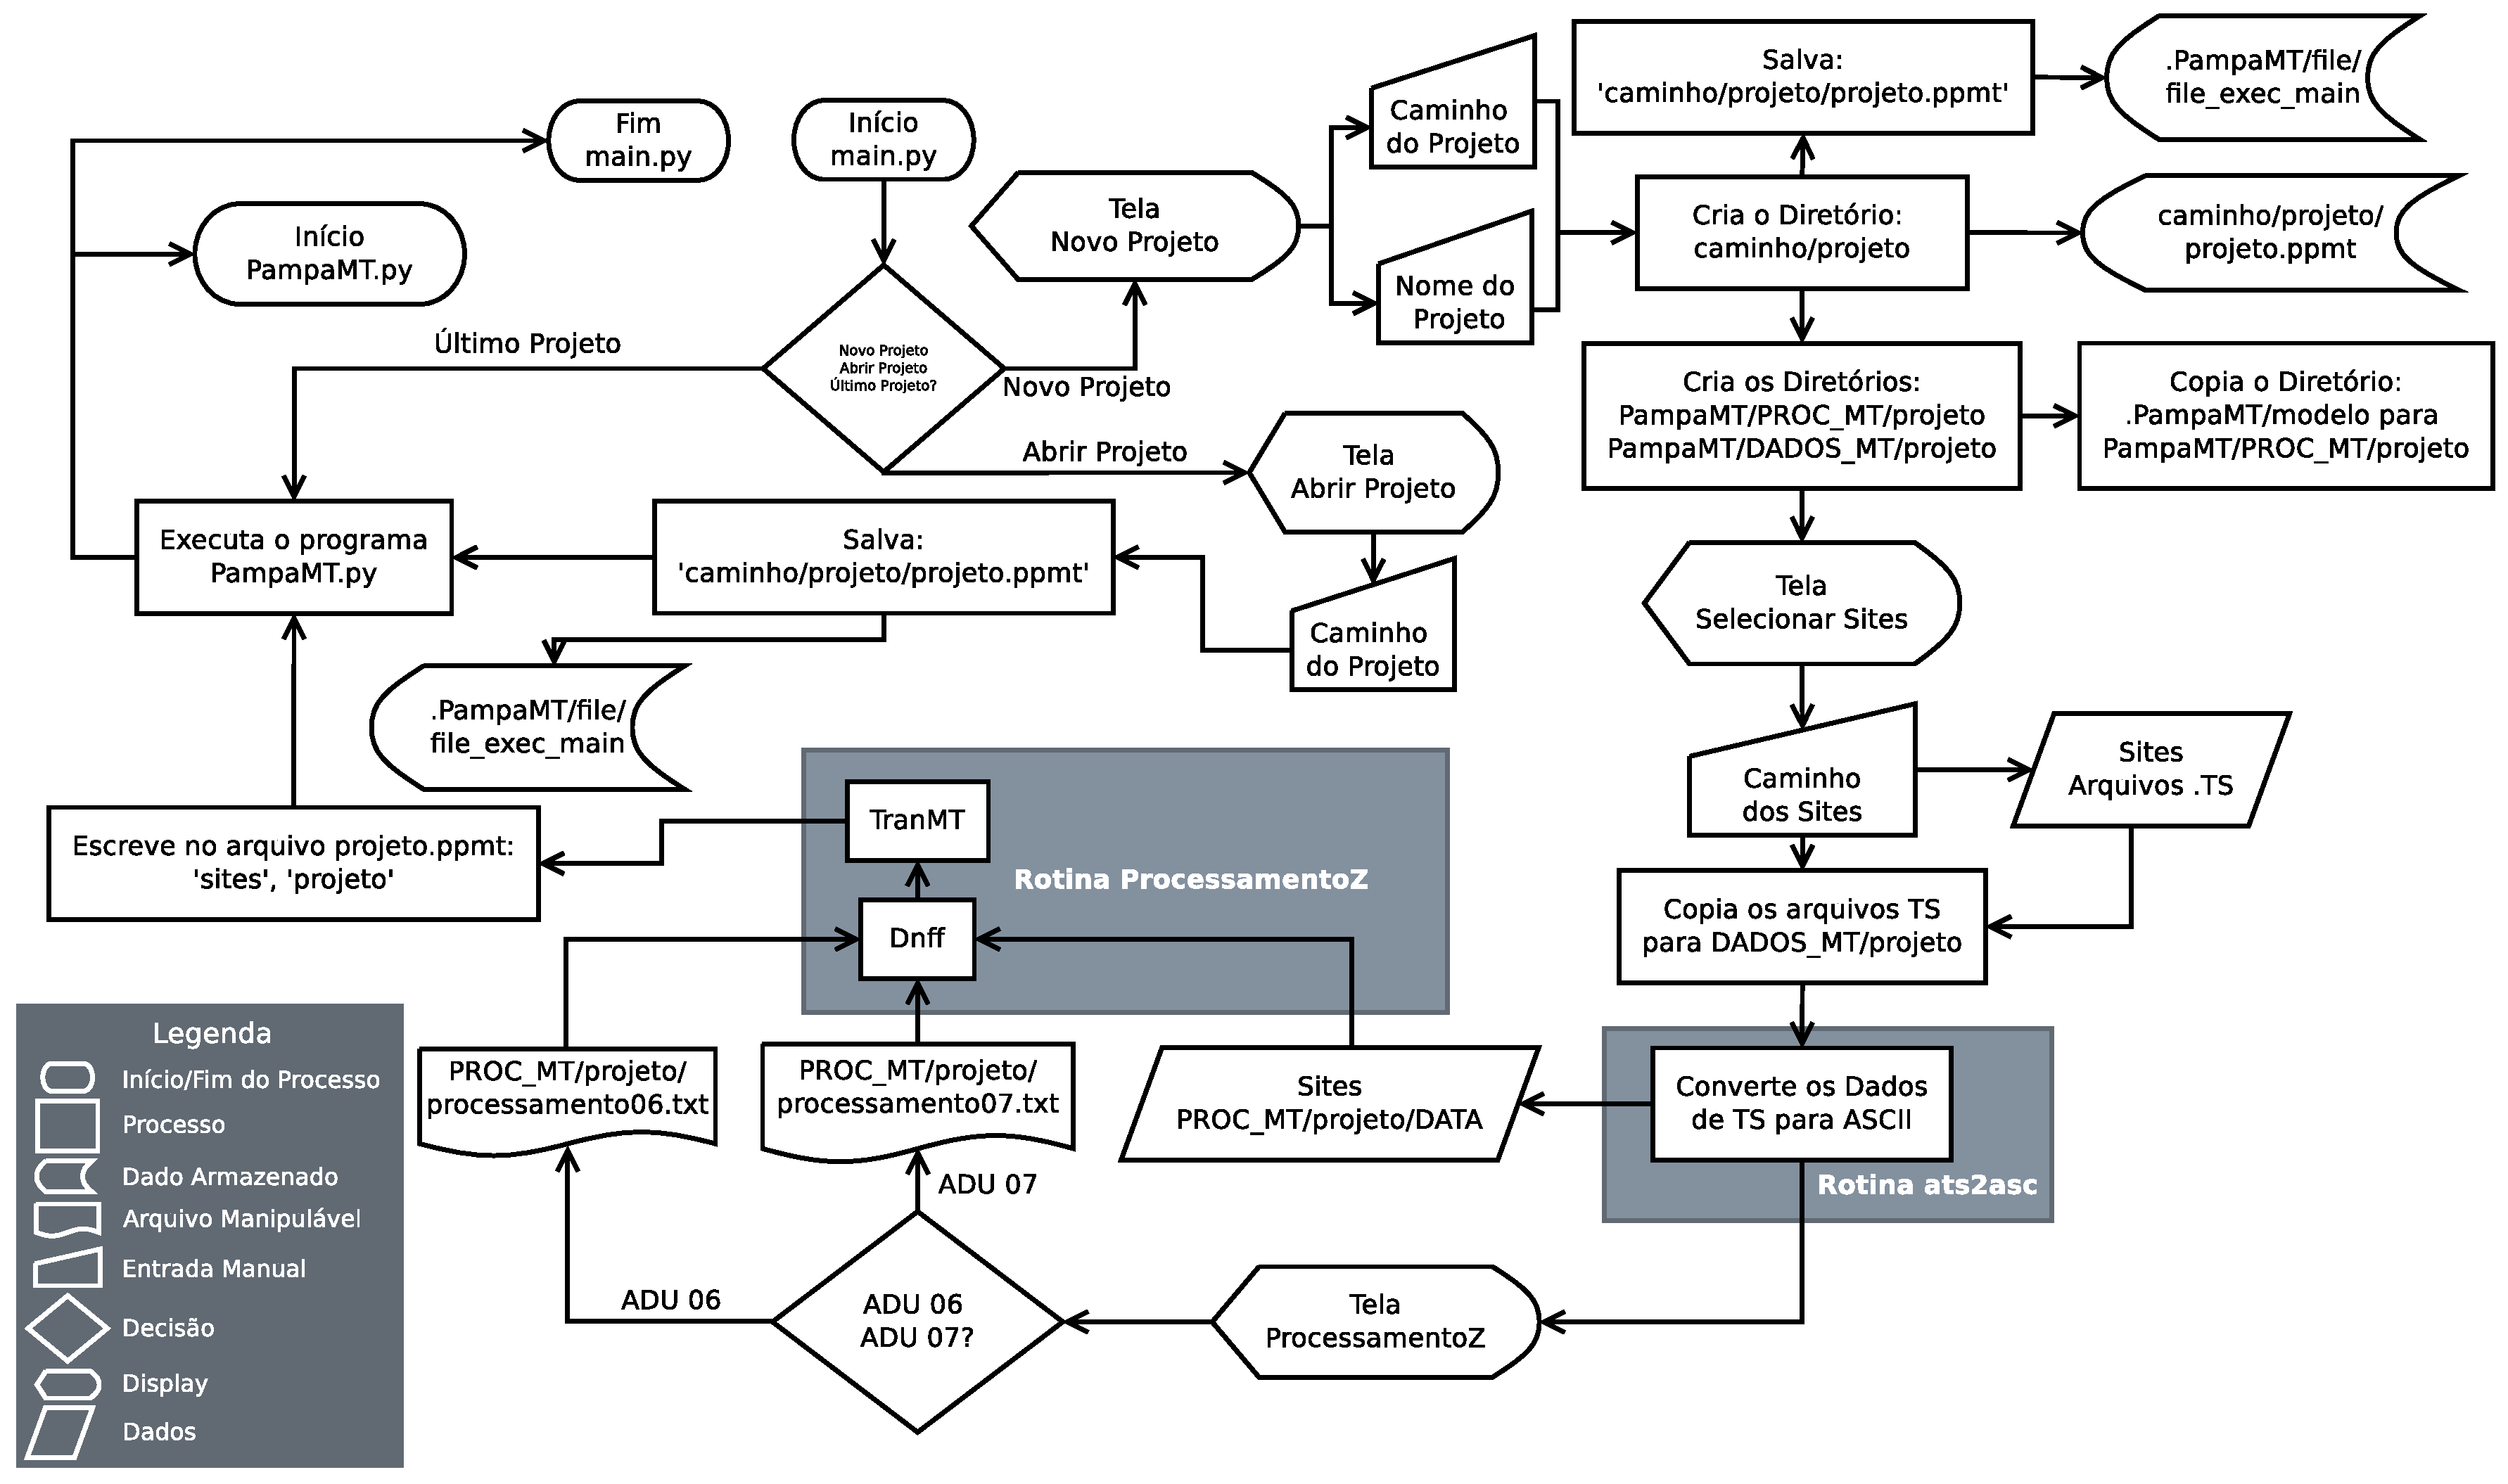
\includegraphics[width=21cm]{texto/fig/mainpy.eps} 
                \end{center}
                \fonte{O Autor, 2018}
                
            \end{figure}
    \end{landscape}%
\lthtmlfigureZ
\lthtmlcheckvsize\clearpage}

\stepcounter{chapter}
\stepcounter{chapter}
\stepcounter{section}
{\newpage\clearpage
\lthtmlpictureA{tex2html_wrap2167}%
\resizebox{\textwidth}{!}{%
                \begin{tabular}{@{}lccccccl@{}}
\toprule
\textbf{Tarefa}  & {\bf Jan}& {\bf Fev}& {\bf Mar}& {\bf Abr}& {\bf Mai}& {\bf Jun} &  \\
\midrule
\par
{\bf 1.} Revisão Bibliográfica 		& 	X  & 	      & 	 & 	    & 	       & 	  \\
\par
{\bf 1.1} Magnetotelúrico      		& 	X  & 	X     & X        & 	    & 	       & 	  \\
%\hline
                        {\bf 1.2} Python 3.5           		& 	   &          & X	 &X 	    & 	       & 	  \\
%\hline
                        {\bf 1.3} Pacote PROC-MT (INPE)           	& 	   & 	      & 	 & 	    & X	       & X	  \\
\par
\bottomrule
\end{tabular}%
                }%
\lthtmlpictureZ
\lthtmlcheckvsize\clearpage}

\stepcounter{section}
{\newpage\clearpage
\lthtmlpictureA{tex2html_wrap2179}%
\resizebox{\textwidth}{!}{%
                \begin{tabular}{@{}lccccccl@{}}
\toprule
\textbf{Tarefa}  & {\bf Jul}& {\bf Ago}& {\bf Set}& {\bf Out}& {\bf Nov}& {\bf Dez} &  \\
\midrule
\par
{\bf 1.} Construção da Interface Gráfica 	 &X 	    & X	       & 	  & 	     & 	        & 	   \\
\par
{\bf 2.} Desenvolvimento dos Scripts         & 	    & 	       & X	  & 	     & 	        & 	   \\
\par
{\bf 3.} Fase de testes com Dados Sintéticos & 	    & 	       & 	  & X	     & 	        & 	   \\
\par
{\bf 4.} Fase de testes com Dados Reais      & 	    & 	       & 	  & 	     &X	        & 	   \\
\par
{\bf 5.} Liberação do Código                 & 	    & 	       & 	  & 	     & 	        & X	   \\
\par
\bottomrule
\end{tabular}%
                }%
\lthtmlpictureZ
\lthtmlcheckvsize\clearpage}



\setlength{\labelsep}{0pt}%

\setlength{\labelsep}{0pt}

\end{document}
